\section{Regular expressions and finite automatons}

%% \todo[inline]{MAn bruger dem til at beskrive tekststrenge med bestemte
%% mønstre, prøv at sætte noget lettere fordøjeligt ind før definitionerne}

A regular language is a possibly infinite set of finite sequences of
symbols from a finite alphabet.

A formal definition of regular languages:
\begin{definition}[Regular language]
  The regular language over the alphabet $\Sigma$ is defined
  recursively as:
  \begin{itemize}
  \item The empty language $\emptyset$.
  \item The empty string language $\{\upvarepsilon\}$.
  \item The singleton language $\{a\}$, for any symbol $a\in \Sigma$.
  \item If $L_r$ and $L_s$ are both regular languages then the union
    $L_r \cup L_s$ is also a regular language.
  \item If $L_r$ and $L_s$ are both regular languages then the
    concatenation $L_r \bullet L_s$ is also a regular language.
  \item if $L$ is a regular language then the Kleene star $L*$ is also
    a regular language.
  \end{itemize}
\end{definition}


\subsection{Regular expressions}

Regular expressions are used to denote regular languages. They are
written in a formal language consisting of two types of characters:
Meta characters and literal characters. The meta characters have
special meaning and are interpreted by a regular expression
engine. The basic meta characters are parenthesis, the alternation
operator and the Kleene star. Parenthesis provides grouping,
alternation allows the choice between different text strings and the
Kleene star repeats. The literal characters have no special meaning
and match literally.

%% \begin{definition}[Regular language]
%% A regular language over the alphabet $\Sigma$ can be defined
%% recursively as follows:
%% \begin{description}
%% \item[Basis clauses] 
%%   \begin{itemize}
%%   \item The empty language $\emptyset$
%%   \item The empty string language $\{\upvarepsilon\}$
%%   \item The singleton language $\{a\}$, for any symbol $a\in \Sigma$
%%   \end{itemize}
%%   are all regular languages
%% \item[Inductive clauses]
%%   If $L_r$ and $L_s$ are both regular languages then
%%   \begin{itemize}
%%   \item The union $L_r \cup L_s$
%%   \item The concatenation $L_r \bullet L_s$
%%   \item The kleene star $L_r*$ 
%%   \end{itemize}
%%   are all regular languages
%% \item[Extremal clause] No other languages over $\Sigma$ are regular
%% \end{description}
%% \end{definition}

%% Regular expressions are used to regular languages:

A formal definition of regular expressions:
\begin{definition}[Regular expression]
  \label{def:regexp}
  A regular expression over an alphabet $\Sigma$ can be defined as follows:
\begin{itemize}
\item An empty string, $\upvarepsilon$, and any character from the
  alphabet $\Sigma$
\item If $r_1$ and $r_2$ are regular expressions, then the
  concatenation $r_1r_2$ are also a regular expression
\item If $r_1$ and $r_2$ are regular expressions, then the alternation
  $r_1|r_2$ is also a regular expression
\item If $r$ is a regular expression, then so is the repetition $r*$
\end{itemize}

Any expression is a regular expression if it follows from a finite
number of applications of the above rules.
\end{definition}

The precedence of the operators are: repetition, concatenation and
alternation, from highest to lowest. Concatenation and alternation are
both left-associative. 

\begin{example}[Regular expression]
  Here we have a somewhat complicated example of a regular expression
  that demonstrates the basic operators.
\label{ex:regular1}
Consider the sentence:
\begin{quote}
\textsl{This book was written using 100\% recycled
  words.}\footnote{Terry Pratchett, Wyrd Sisters}
\end{quote}

Other writings such as papers and novels also use words. If we
want to catch sentences referring to these writings as well, we can
use the regular expression: \texttt{(book|paper|novel)}. 

To match the number 100 in the sentence, we could use the regular
expression \texttt{100}. In most cases however we will not know
beforehand how many words are recycled, so we may want to use the
regular expression \texttt{(0|1|2|3|4|5|6|7|8|9)*}, which will match
any natural number.

With this in mind we can write a regular expression to match our
sentence:
\begin{quote}
  \texttt{This (book|paper|novel) was written using \\
    (0|1|2|3|4|5|6|7|8|9)*\% recycled words.}
\end{quote}

\end{example}

\subsection{Extensions to the regular expressions}

Many tools extend the regular expressions presented in the previous
section. They add new notation to make it easier to specify
patterns. In this section we present the extensions to definition
\vref{def:regexp} we have made: Extra quantifiers, character classes,
a quoting character, a wild card and some non-capturing parenthesis.

\begin{itemize}
\item The quantifier $+$ causes the regular expression $r$ to be
  matched one or more times. This can also be written as $rr*$
\item The quantifier $?$ causes the regular expression $r$ to be
  matched zero or one times. This can also be written as
  $\upvarepsilon|r$
\item A character class is delimited by $[]$ and matches exactly one
  character in the input string. Special characters loose their
  meaning inside a character class; $*$, $+$, $?$, $($, $)$ and so on
  are treated as literals.

  Characters can be listed individually, e.g. \texttt{[abc]}, or they
  can be listed as ranges with the range operator: $-$,
  e.g. \texttt{[a-z]}. These can be rewritten in terms of our original
  regular expression: \texttt{a|b|c} and \texttt{a|b|c...x|y|z}
  respectively.

  To match characters not within the range, the complement operator is
  used. \texttt{\^{}} used as the first character in a character
  class, elsewhere it will simply match literally, indicates that only
  characters not listed in the character class should
  match. E.g. \texttt{[\^{}\^{}]} will match anything but a
  \texttt{\^{}}
\item The quoting character \textsf{\textbackslash} will allow the
  operators to match literally. We use \textsf{\textbackslash *} to
  match a \textsl{*}.
\item The wild card \texttt{.} will match any character, including a
  newline.
\item For the non-capturing parenthesis we have the choice of
  notation. Here we will list some of the options, where $r$ is some
  regular expression:
  \begin{itemize}
  \item The industry standard, to which Perl, Python, RE2 and most
    others adhere is: $(?:r)$.
  \item Perl 6 \cite{Wall2002} suggests use of square parenthesis instead:
    $[r]$. These are however already in use by the character classes.
  \item A more intuitive notation could be using single parenthesis
    for non-capturing, $(r)$, and double parenthesis for capturing,
    $((r))$.
  \item Since we are not using $\{r\}$ as special notation, this could
    be a good use, it surely would be the simplest to implement. This
    is however used in the repetition notation in industry standard.
  \end{itemize}
  
  Since there is a standard, we will adhere to it, and use $(?:r)$ for
  non-capturing parenthesis.
\end{itemize}
\begin{example}

As we saw in example \ref{ex:regular1}, we can match a natural number
with the regular expression \texttt{(0|1|2|3|4|5|6|7|8|9)*}. Using the
expansions to regular expressions above, we can rewrite this as:
\begin{description}
\item[\texttt{[0-9]*}] This literally means the same thing.
\item[\texttt{[0-9]+}] We can use a different repetition operator and
  require there be at least one digit.
\item[\texttt{[1-9][0-9]*}] This matches any natural number as
  well, but it will not match any preceding zeros. This is a
  refinement, in that it will match fewer text strings than the first
  expression. This is however not always an advantage.
\end{description}
\end{example}


\subsection{Finite automatons}

Finite automatons are used to solve a wide array of problems. In this
thesis we will focus on finite automatons as they are used with
regular expressions. A finite state machine consists of a number of
states and transitions between states. One state is marked as the
initial state, a set of states is marked as final. To each transition
there is attached a condition. Input is consumed in sequence, for each
symbol transitions are taken when their attached condition are met. If
the simulation ends in a final state, the finite automaton is said to
accept the input.

Finite automatons can be divided in two categories: The deterministic
(DFA) and the non-deterministic (NFA) finite automaton. This
distinction is mostly relevant in practice, as they are
equivalent. NFAs and DFAs recognize exactly the regular languages.


\begin{description}
\item[NFA] For each pair of input symbol and state, there may be more
  than next states. This means that there may be more than one path
  through an NFA for an input string.

  The $\upvarepsilon$-transitions are an extension of the NFA. These
  are special transitions that can be taken without consuming any
  input symbols. This also has mainly practical implications, NFAs
  with and without $\upvarepsilon$-transitions are equivalent.

\item[DFA] For each pair of input symbol and state, there may be only
  one next state. This means there is only one path through the DFA
  for an input string.
\end{description}

\subsection{Regular expression to NFA}
\label{sec:from_regular_expression_to_nfa}
Every regular expressions can be converted to a NFA matching the same
language.  This section will describe an approach to doing so.

\subsubsection{Thompson}
\label{sec:re2nfa_thompson_theory}
The method described in this section first appeared in Ken Thompsons
article from 1968 \cite{Thompson1968}. The descriptions given in for
example \cite{HopcroftJohnE.AndMotwaniRajeevAndUllman2001},
\cite{Aho:1986:CPT:6448} and \cite{RussCox} are considered more
readable and we will be basing our description on these.

The NFA will be build in steps from smaller NFA fragments. A NFA
fragment has an initial state, but no accepting state, instead it has
one or more dangling edges leading nowhere (yet).


%% a method for converting a
%% regular expression to an automaton is described. The method works by
%% breaking the regular expression up into fragments; Each fragment also
%% being a regular expression in itself. Using this method yields an
%% automaton with the following characteristics:
%% \begin{itemize}
%% \item There is exactly one initial state
%% \item There are no edges into the initial state
%% \item There is exatly one accepting state
%% \item There are no edges out of the accepting state
%% \item There are at most two edges leaving a state
%% \end{itemize}

The base fragment corresponds to the regular expression consisting
only of a single character \textit{a}. The NFA fragment is shown in
figure \vref{fig:basecase1}. One state with a single edge, marked with
the character \textit{a} is added. The new state is the initial state
for this fragment and the edge is left dangling.

\begin{figure}
  \centering
  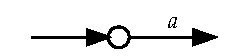
\includegraphics{parsing/basecase1}
  \caption{Fragment accepting a single character \textit{a}}
  \label{fig:basecase1}
\end{figure}

The second base fragment corresponds to the empty regular
expression. The NFA fragment is shown in figure
\vref{fig:basecase4}. One state with a single edge marked as a
$\upvarepsilon$-edge is added. The new state is the initial state for
this fragment and the edge is left dangling. This fragment is used for
the empty regular expression and for alternations with one or more
options left empty.

%% In Ken Thompson article from 1968 \cite{Thompson1968}, in
%% \cite{HopcroftJohnE.AndMotwaniRajeevAndUllman2001} and in
%% \cite{RussCox} a method for converting a regular expression to an
%% automaton is described.



%% The base case is the regular expression consisting of a single
%% character \textit{a}. Figure \vref{fig:basecase1} shows an automaton
%% accepting the same language. 

\begin{figure}
  \centering
  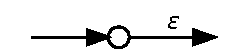
\includegraphics{parsing/basecase4}
  \caption{Fragment accepting the empty string}
  \label{fig:basecase4}
\end{figure}


%% \begin{figure}
%%   \centering
%%   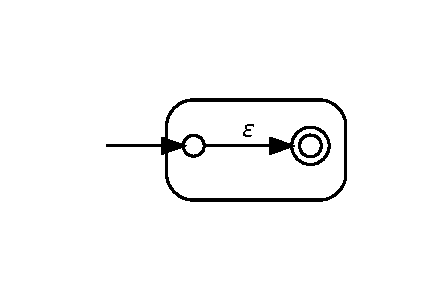
\includegraphics{parsing/basecase3}
%%   \caption{The empty string}
%%   \label{fig:basecase3}
%% \end{figure}

The first compound fragment is alternation, see figure
\vref{fig:alternation}. Here, the two sub-fragments R and S are automatons
with initial states and some dangling edges. What else they are
composed of, is irrelevant for the moment\todo{changed}. We add one new state, 
and make it the initial state for this fragment. The initial state has two
$\upvarepsilon$-edges leaving, connecting to the initial states of R
and S. The dangling edges for the new fragment is the sum of the
dangling edges leaving R and S.

\begin{figure}
  \centering
  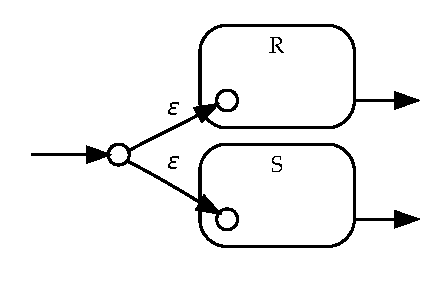
\includegraphics{parsing/alternation}
  \caption{Alternation R\textbar S}
  \label{fig:alternation}
\end{figure}

Concatenation of two regular expressions R and S is achieved as shown
in figure \vref{fig:concatenation}. The dangling edges of R is
connected to the initial state of S. The initial state for the new
fragment is the initial state of R and the dangling edges of S is
still left dangling.

\begin{figure}
  \centering
  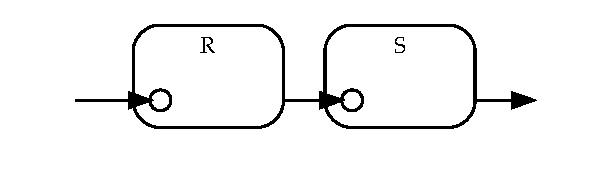
\includegraphics{parsing/concatenation}
  \caption{Concatenation RS}
  \label{fig:concatenation}
\end{figure}

Zero or more times repetition is shown in figure
\vref{fig:repetition}. One new, initial, state is added. It has two
$\upvarepsilon$-edges leaving, one is connected to the initial state of
R and one is left dangling. The dangling edges of R is connected to
the new initial state.

\begin{figure}
  \centering
  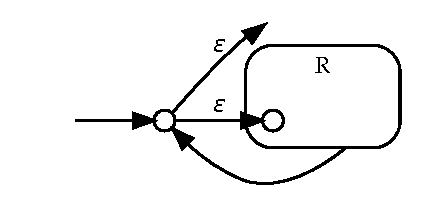
\includegraphics{parsing/repetition}
  \caption{Repetition R*}
  \label{fig:repetition}
\end{figure}

Finally an accepting state is patched into the NFA. All edges left
dangling is connected to the accepting state. 

\paragraph{Properties} NFAs created with Thompsons method has these
properties:
\begin{itemize}
  \item At most two edges is leaving a state
  \item There are no edges leaving the accepting state
  \item There are no edges leading into the starting state
\end{itemize}


\begin{example}[Converting a regular expression to a NFA]
\label{ex:converting_a_regular_expression_to_a_nfa}
\begin{figure}
  \centering 
  \subfigure[Fragment for \textsf{a}]{
    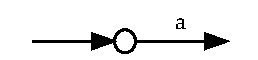
\includegraphics{parsing/ex_a.pdf}
    \label{fig:ex_parsing_a}
  }
  \subfigure[Fragment for \textsf{b}]{
    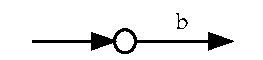
\includegraphics{parsing/ex_b.pdf}
    \label{fig:ex_parsing_b}
  }
  \subfigure[Fragment for \textsf{c}]{
    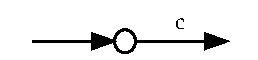
\includegraphics{parsing/ex_c.pdf}
    \label{fig:ex_parsing_c}
  }
  \subfigure[Fragment for \textsf{a*}]{
    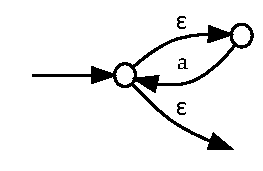
\includegraphics{parsing/ex_star.pdf}
    \label{fig:ex_parsing_star}
  }
  \subfigure[Fragment for \textsf{a*b}]{
    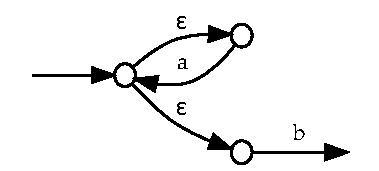
\includegraphics{parsing/ex_concat.pdf}
    \label{fig:ex_parsing_concat}
  }
  \subfigure[Fragment for \textsf{a*b\textbar c}]{
    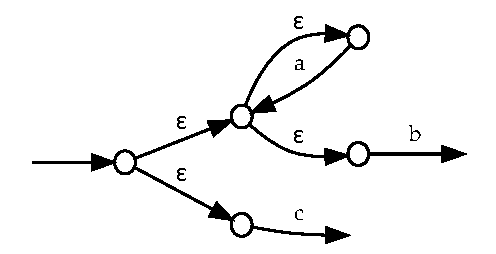
\includegraphics{parsing/ex_alt.pdf}
    \label{fig:ex_parsing_alt}
  }
  \subfigure[Final NFA for \textsf{a*b\textbar c}]{
  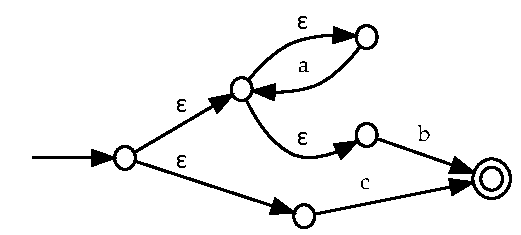
\includegraphics{parsing/ex_finished.pdf}
  \label{fig:ex_parsing_finished}
  }
  \caption{Individual fragments when converting \textsf{a*b\textbar c}
    to NFA}
  \label{fig:ex_parsing}
\end{figure}

\begin{figure}
\end{figure}


In this example we will be converting the regular expression
\textsf{a*b\textbar c} to a NFA using Thompsons method.
\begin{itemize}
\item Top level we have the alternation operator, but before we can
  complete this fragment, we need to convert \textsf{a*b} and
  \textsf{c} to fragments.
  \begin{itemize}
  \item \textsf{a*b} is complicated since we have one operator, two
    literals and a hidden concatenation. Top level we have the
    concatenation operator, concatenating \textsf{a*} and
    \textsf{b}. These needs to be converted before we can concatenate.
    \begin{itemize}
    \item \textsf{a*} needs to be broken further down. Top level we have
      the Kleene star, but we can not apply the rule for converting this
      to a NFA fragment before we have converted \textsf{a}. 
      \begin{itemize}
        \item \textsf{a} is straightforward, we just apply the rule
          for transforming literals and we have the fragment in figure
          \ref{fig:ex_parsing_a}
      \end{itemize}
      Using this fragment to complete the Kleene star, we have the
      fragment in figure \ref{fig:ex_parsing_star}.
    \item \textsf{b} is straightforward, we just apply the rule for
      transforming literals and we have the fragment in figure
      \ref{fig:ex_parsing_b}.
    \end{itemize}
    Now we are ready to concatenate, fragments
    \ref{fig:ex_parsing_star} and \ref{fig:ex_parsing_b} are
    concatenated and we have the fragment in figure \ref{fig:ex_parsing_concat}
  \item \textsf{c} is straightforward, we just apply the rule for
    transforming literals and we have the fragment in figure
    \ref{fig:ex_parsing_c}.
  \end{itemize}
  With these expressions converted to fragments we can apply the
  alternation conversion rule. We have the resulting fragment in
  figure \ref{fig:ex_parsing_alt}
\end{itemize}

All that is left now is to connect the dangling edges to an accepting
state. We have the final result in figure \vref{fig:ex_parsing_finished}
  
\end{example}

\subsection{Matching}

The NFAs constructed as described in section
\vref{sec:from_regular_expression_to_nfa} can be used to match a
regular expression with a string, i.e. to determine if a string belongs
to the language of the regular expression. 

Once the NFA is generated, simulating it is a straightforward
task. Again, our method is attributed to Thompson
\cite{Thompson1968}. 
\begin{enumerate}
    \item We maintain a set of active states and a pointer
    to the current character in the string
    \item At the beginning only the
    start state belongs to the set of active states
    \item The string is read
    from left to right, taking each character in turn. When a character is
    read from the input string, all legal transitions from the states in
    the active set is followed
    \item A transition is legal if it is a
    $\upvarepsilon$-transition or if the mark on the transition matches
    the character read from the input string. The new set of active states
    is the set of end states for the transitions followed
    \item If the
    accepting state is included in the active set when the string is read,
    the string matches the regular expression
\end{enumerate}

With this method we only ever add a state to the active set once per
iteration and we only read each character from the input string once.


\begin{example}[Matching with a NFA]
  \begin{figure}
    \centering
    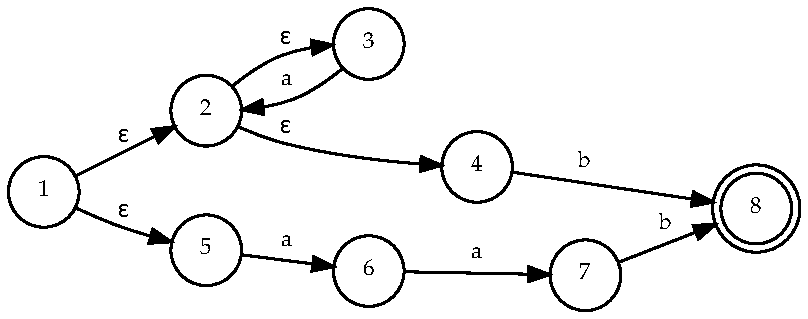
\includegraphics[width=\textwidth]{matching/ex_matching.pdf}
    \caption{NFA for the regular expression \textsf{a*b\textbar aab}}
    \label{fig:ex_matching}
  \end{figure}
  
  In this example we will demonstrate how the regular expression
  \textsf{a*b\textbar aab} is matched with the string \textsl{aab}. In
  figure \vref{fig:ex_matching} we have the corresponding NFA. Each
  state is marked with a unique number which we will be referring to
  in the table below.

\begin{center}
\begin{tabular}{ccp{8.5cm}}
Active set & \texttt{SP} & Explanation \\
\hline

1 & \textsl{\underline{a}ab} & Initially we have the start state in
the active set and \texttt{SP} points to the start of the string. \\

3, 4, 5 & \textsl{\underline{a}ab} & Following all
$\upvarepsilon$-transitions. \\

2, 6 & \textsl{a\underline{a}b} & Reading the first \textsl{a} from the input
string, states 3 and 5 have legal transitions on \textsl{a}. \\

3, 4, 6 & \textsl{a\underline{a}b} & Following all
$\upvarepsilon$-transitions. \\

2, 7 & \textsl{aa\underline{b}} & Reading the second \textsl{a} from
the input string, states 3 and 6 have legal transitions on
\textsl{a}. \\

3, 4, 6 & \textsl{aa\underline{b}} & Following all
$\upvarepsilon$-transitions. \\

8 & \textsl{aab\underline{ }} & Reading the last character from input
string: \textsl{b}, states 4 and 7 have legal transitions on
\textsl{b}. \\

8 & \textsl{aab\underline{ }} & No $\upvarepsilon$-transitions to follow.

\end{tabular}
\end{center}

After reading the string we can see that the accepting state is in the
active set: We have a match!

\end{example}



\subsection{Summary}

Regular expressions are a widely used and popular tool. The features
offered and the semantics vary. For example some will offer
backreferencing and others will not, some will offer a leftmost match
in alternations others will offer a longest match. The underlying
implementation and performance vary widely. A regular expression
engine will solve some problems more efficiently than others.

%% \todo[inline]{write something about how regular expressions can be
%%   very powerful but the underlying design and its performance can vary
%% widely}
